\section{Biological Applications}
\label{sec:biological-applications}
\subsection{Biological Applications I}
\label{subsec:biological-applications-1}
\begin{frame}{\insertsubsection}
    % \begin{table}
    %     \centering
    %     \makegapedcells
    %     \begin{tabular}{@{}lcccc@{}}
    %         \toprule
    %         Input Data
    %         \cmidrule{1-5}
    %         
    %         \bottomrule
    %     \end{tabular}
    %     \caption{Different applications in Biological contexts.}
    %     \label{tab:biological-applications-table-1}
    % \end{table}
    \begin{figure}
        \centering
        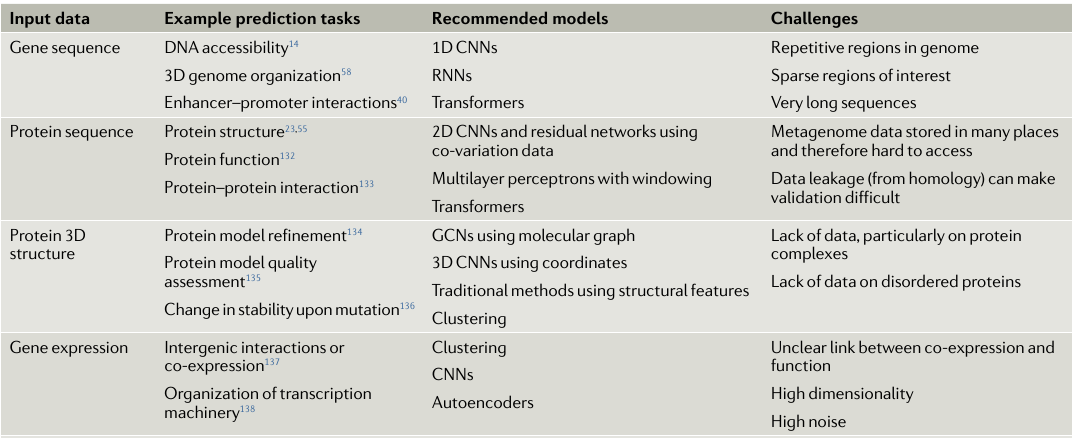
\includegraphics[width=\textwidth]{media/table_1.png}
        \caption{Different applications in Biological contexts. I}
    \end{figure}
\end{frame}
%
%
\begin{frame}{\insertsubsection}
    \begin{figure}
        \centering
        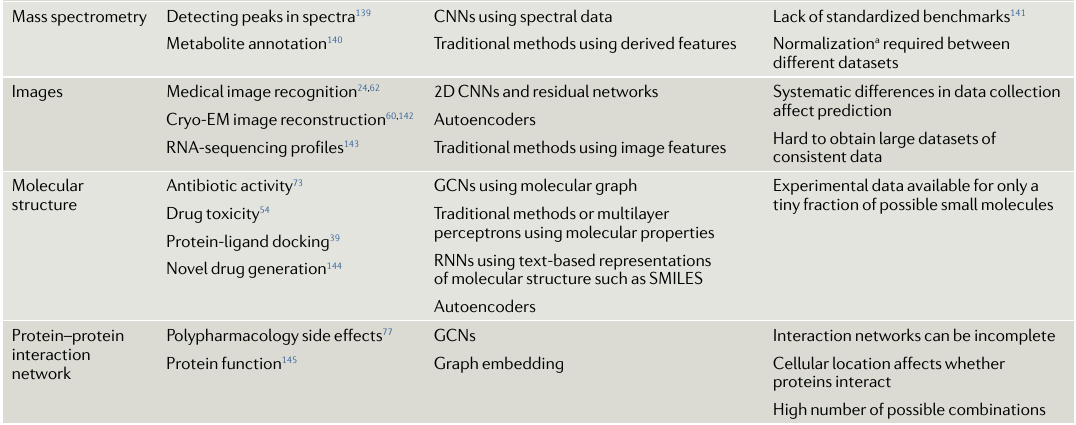
\includegraphics[width=\textwidth]{media/table_2.png}
        \caption{Different applications in Biological contexts. II}
    \end{figure}
\end{frame}